\chapter{Introduction}

Information Visualization is the field of study concerned with providing visual tools to improve our reasoning about abstract data. Abstract data has no physical representation or direct spatial association, such as data tables, relational databases, and graphs.
In this thesis, we will focus on testing and improving visualization techniques designed to portray two specific kinds of abstract datasets: \emph{temporal hierarchical} and \emph{temporal multidimensional}.

\eduardo{add necessary refs later}

\section{Temporal hierarchical data and treemaps}

Hierarchical datasets are trees with weighted nodes. Weights are given for leaf nodes and computed for non-leaf nodes as the sum of their children's weights. One example of a hierarchical dataset is a computer's file system -- the "shape of the tree" is given by the organization of the directories, and the weight of the leaf nodes can be defined as a file attribute such as size.
The temporal aspect is introduced when data changes over time. Building upon the file system example, if we collect "snapshots", as in a git repository or periodic backups of a hard drive, our data would be an evolving tree -- its organization (hierarchy) changes as we create and delete folders and files, and the weight of the leaf nodes change as files are edited.

There is a range of visual encodings suitable/designed for displaying hierarchical data, including node-link diagrams, icicle plots, sunburst plots, and, the focus of our research, \emph{treemaps}.

Given an input weighted tree, treemaps recursively partition a 2D spatial region into cells whose area (and possibly color, shading, and labels) encode the tree's data attributes. 
Connecting back to our initial example, the first treemaping algorithm was, in fact, designed for the purpose of displaying the contents and use of a file system by Ben Shneiderman:

\begin{quoting}
    "During 1990, in response to the common problem of a filled hard disk, I became obsessed with the idea of producing a compact visualization of directory tree structures. Since the 80 Megabyte hard disk in the HCIL was shared by 14 users it was difficult to determine how and where space was used. Finding large files that could be deleted, or even determining which users consumed the largest shares of disk space were difficult tasks".
\end{quoting}

Compared to other hierarchical visualization methods, treemaps scale well, making use of all available screen pixels to show data and thus able to handle trees of thousands of nodes. As Shneiderman realized when trying to reason and make decisions about the use of space in his lab's hard drives:
\textit{"Tree structured node-link diagrams grew too large to be useful, so I explored ways to show a tree in a space-constrained layout."}

Over the years, a range of different treemaping techniques was proposed, each designed to optimize different goals such as cell aspect ratio of cells (tied to readability), order preservation, similarity-based placement, and portrayal of uncertainty. The most common form of treemaps are rectangular treemaps, but a range of alternative models exist, such as Voronoi treemaps, Orthoconvex and L-shaped treemaps, and Jigsaw treemaps.
Yet, not much work has been done regarding dynamic treemaps, that is, treemap methods designed to portray temporal hierarchical datasets ensuring that temporal coherence is kept.

% \begin{figure*}[]
%     \centering
%     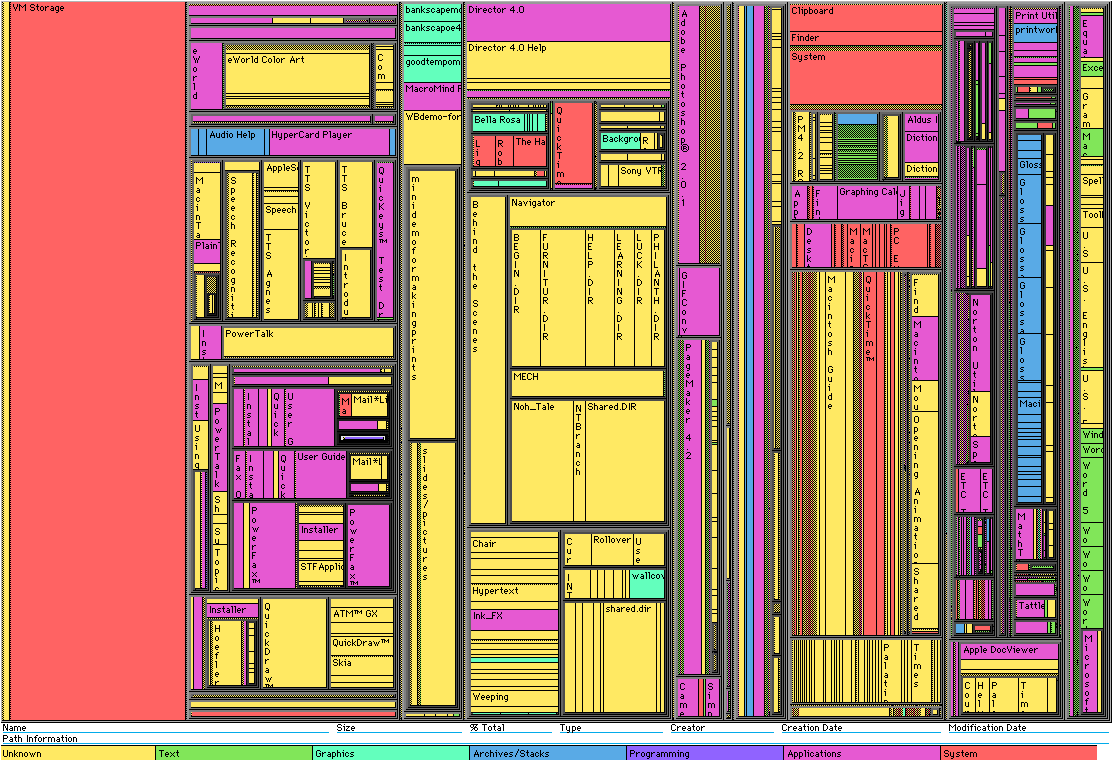
\includegraphics[width=.8\textwidth]{figures/intro/treemap_snd_colorful.png}
%     \caption{Earliest treemap method, Slice-and-Dice, displaying a file system.}
% \end{figure*}

\section{Temporal multidimensional data and projections}

Multidimensional (or high-dimensional) datasets have a number of observations (also called points or samples) where each observation has many attributes, also called variables, dimensions, or measurements. 

For datasets with relatively small numbers of observations and dimensions, techniques such as glyphs, parallel coordinate plots, table lenses, and scatterplot matrices may produce accurate and useful visual encodings.  
If a dataset has a large number of dimensions, however, multidimensional projections tend to be the only scalable approach.  

Traditionally, multidimensional projections take data in a high-dimensional space and project it into a lower-dimensional space, usually creating a 2D or 3D scatter plot, which we can visualize and reason about. In this transformation, the projection method attempts to create visual patterns that reflect the similarities or structure found in the high-dimensional space.

To "reflect the similarities or structure found in the high-dimensional space" can be interpreted in many ways, and the search for the "best" projection method has led to the proposal of an enormous number of techniques.
There are many desirable traits projection methods can have, such as creating high distance/neighborhood preservation maps, scalability, simplicity, interpretability, out-of-sample capability, stability, among others. 
Optimizing a single one of these traits is already a great task that requires tradeoffs regarding the remaining traits and no single current method optimally satisfies all desirable requirements.

The trait that concerns us most in this thesis is stability. Stability, or temporal coherence, needs to be taken into account when we project \emph{temporal} multidimensional data, that is, when the multidimensional data changes over time and, as illustrated in the previous section, we have multiple "snapshots" of the data. 
Most such techniques are designed for static data, and when used for time-dependent data, they usually fail to create a stable and suitable low dimensional representation.

\section{Temporal coherence}

Treemaps and projections are incredibly useful techniques that, due to their compact and easy to interpret design, give unique insights into large and complicated datasets.
They were initially designed for static datasets, but, naturally, if given a temporal hierarchical or multidimensional dataset, we would like to use their concise power of expression to visualize the data. However, when creating these animation-like encodings, since these methods are not designed to maintain temporal coherence, they may create deceitful visual changes and algorithm-driven artifacts.

To illustrate dynamic projection instability, Fig.~\ref{fig:intro-pj-demo-instability} shows three different methods (G-PCA, TF-PCA, and TF-tSNE) projecting the same dataset, using a trail-like visual encoding. The \emph{gaussians} dataset is a 100-dimensional dataset of 2000 samples covering 10 distinct isotropic Gaussian distributions that collapse into 10 single points over 10 timesteps. Knowing the dataset, we can tell that G-PCA renders quite faithfully the data dynamics and structure; TF-PCA creates an artificial amount of spiraling; and TF-tSNE creates a very large amount of apparently random and unstable motion that is not present in the data.  


% https://docs.google.com/drawings/d/1XENnHkpmsl6AqJfx5l2b-H4bSuKonbjgjYY_E599Q5c/edit
\begin{figure*}[h]
    \centering
    \includegraphics[width=\linewidth]{figures/projection-algorithm/demo-instability-trails-rebuttal-with-color-3.eps}
   %  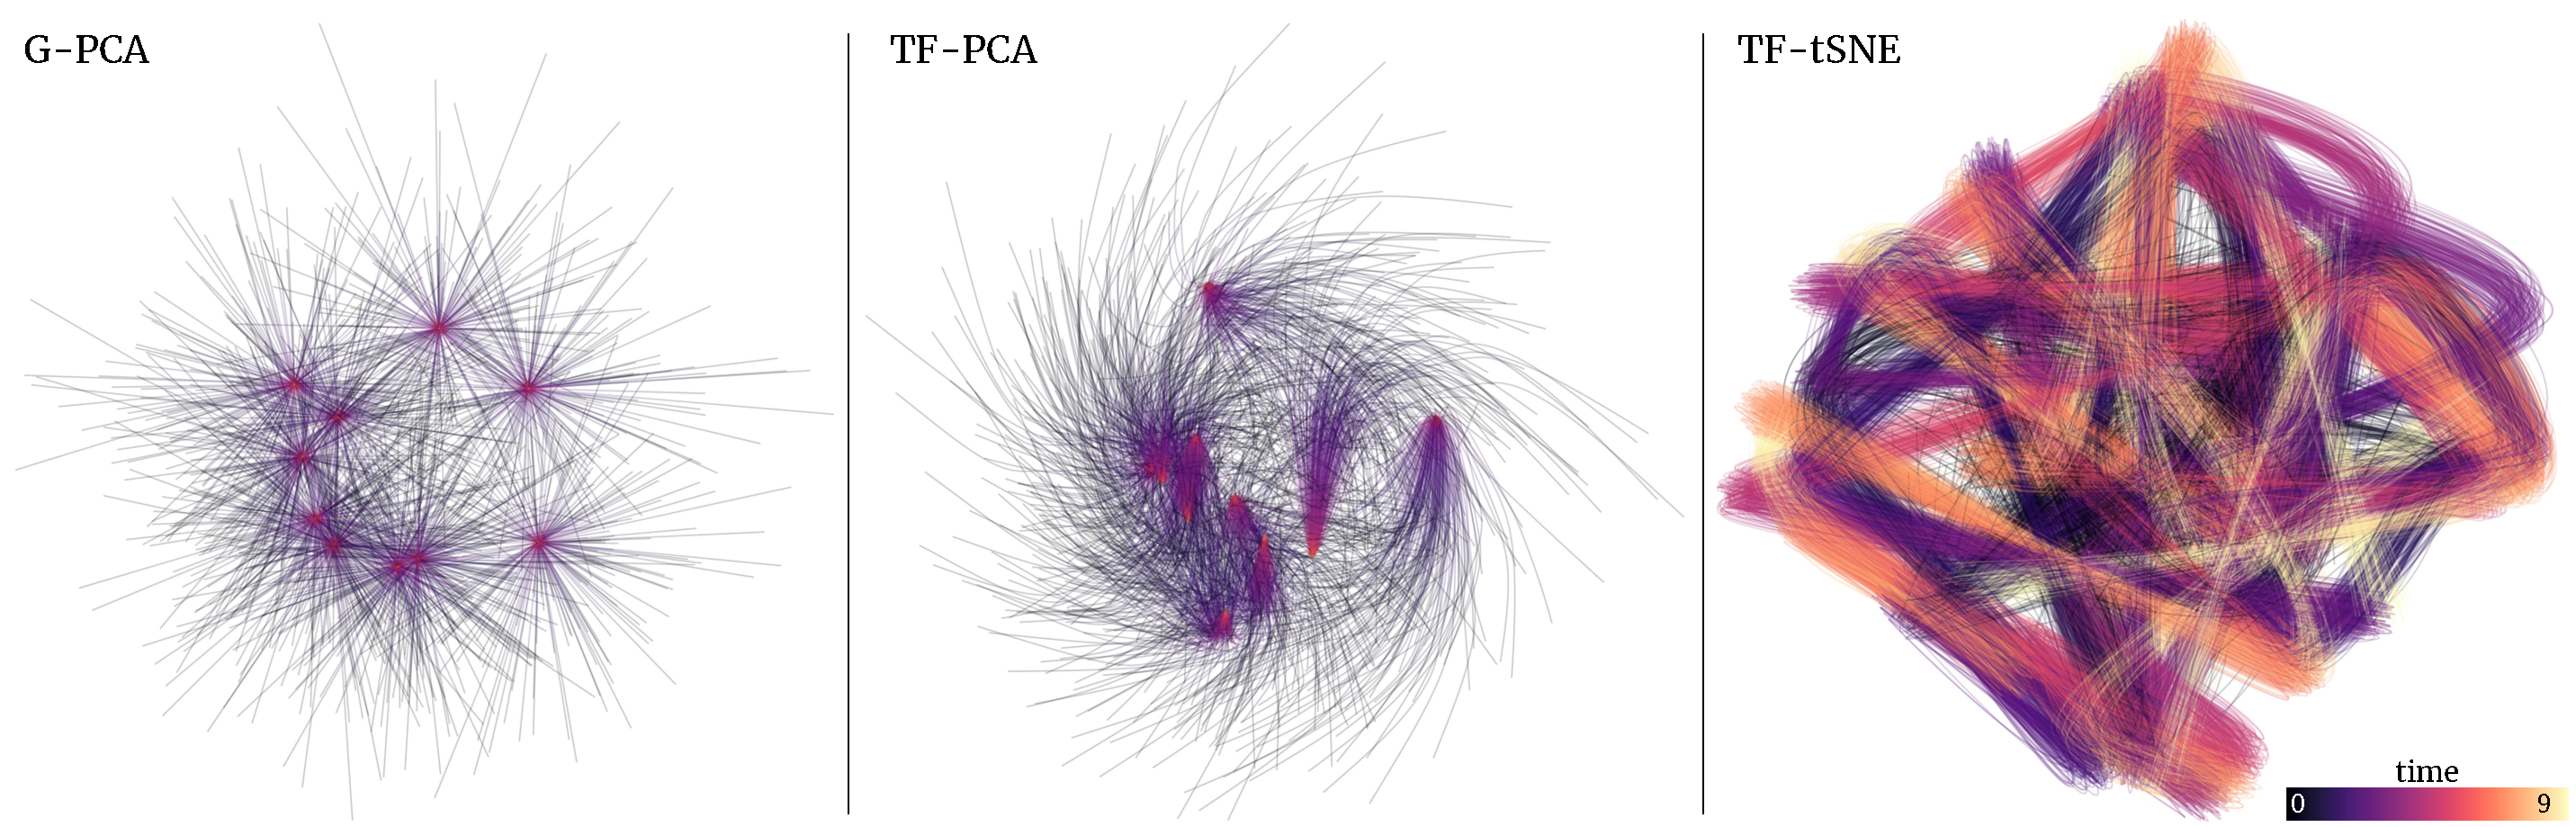
\includegraphics[width=0.48\linewidth]{figures/projection-algorithm/demo-instability-trails-rebuttal-with-color.pdf}
    \caption{A time-dependent collapsing 100-dimensional 10-Gaussian-distributions dataset (2000 points) is visualized by three projection methods. Point trails are colored by time (top) and class (bottom). The images show increasing amounts of instability artefacts.}
    \label{fig:intro-pj-demo-instability}
\end{figure*}

The same effect occurs when we create time-dependent treemaps. The top row of Fig.~\ref{fig:intro-tm-demo-instability} shows three snapshots/timesteps of the evolution of a simple weighted tree, and the next two rows show two different treemapping algorithms creating rectangular treemap representations for the data.
Notice that Nmap creates a stable layout; that is, there are no significant changes in the positions of the cells driven by the small changes in the data, and the adjacencies in the layout remain the same over the evolution.
While in the Squarified treemap layout, cell \emph{d} (red) keeps changing its relative position. When dealing with more complicated datasets, this movement can happen for multiple cells simultaneously, making it impossible to reason about the data and the change in the data.

\begin{figure*}[h]
    \centering
    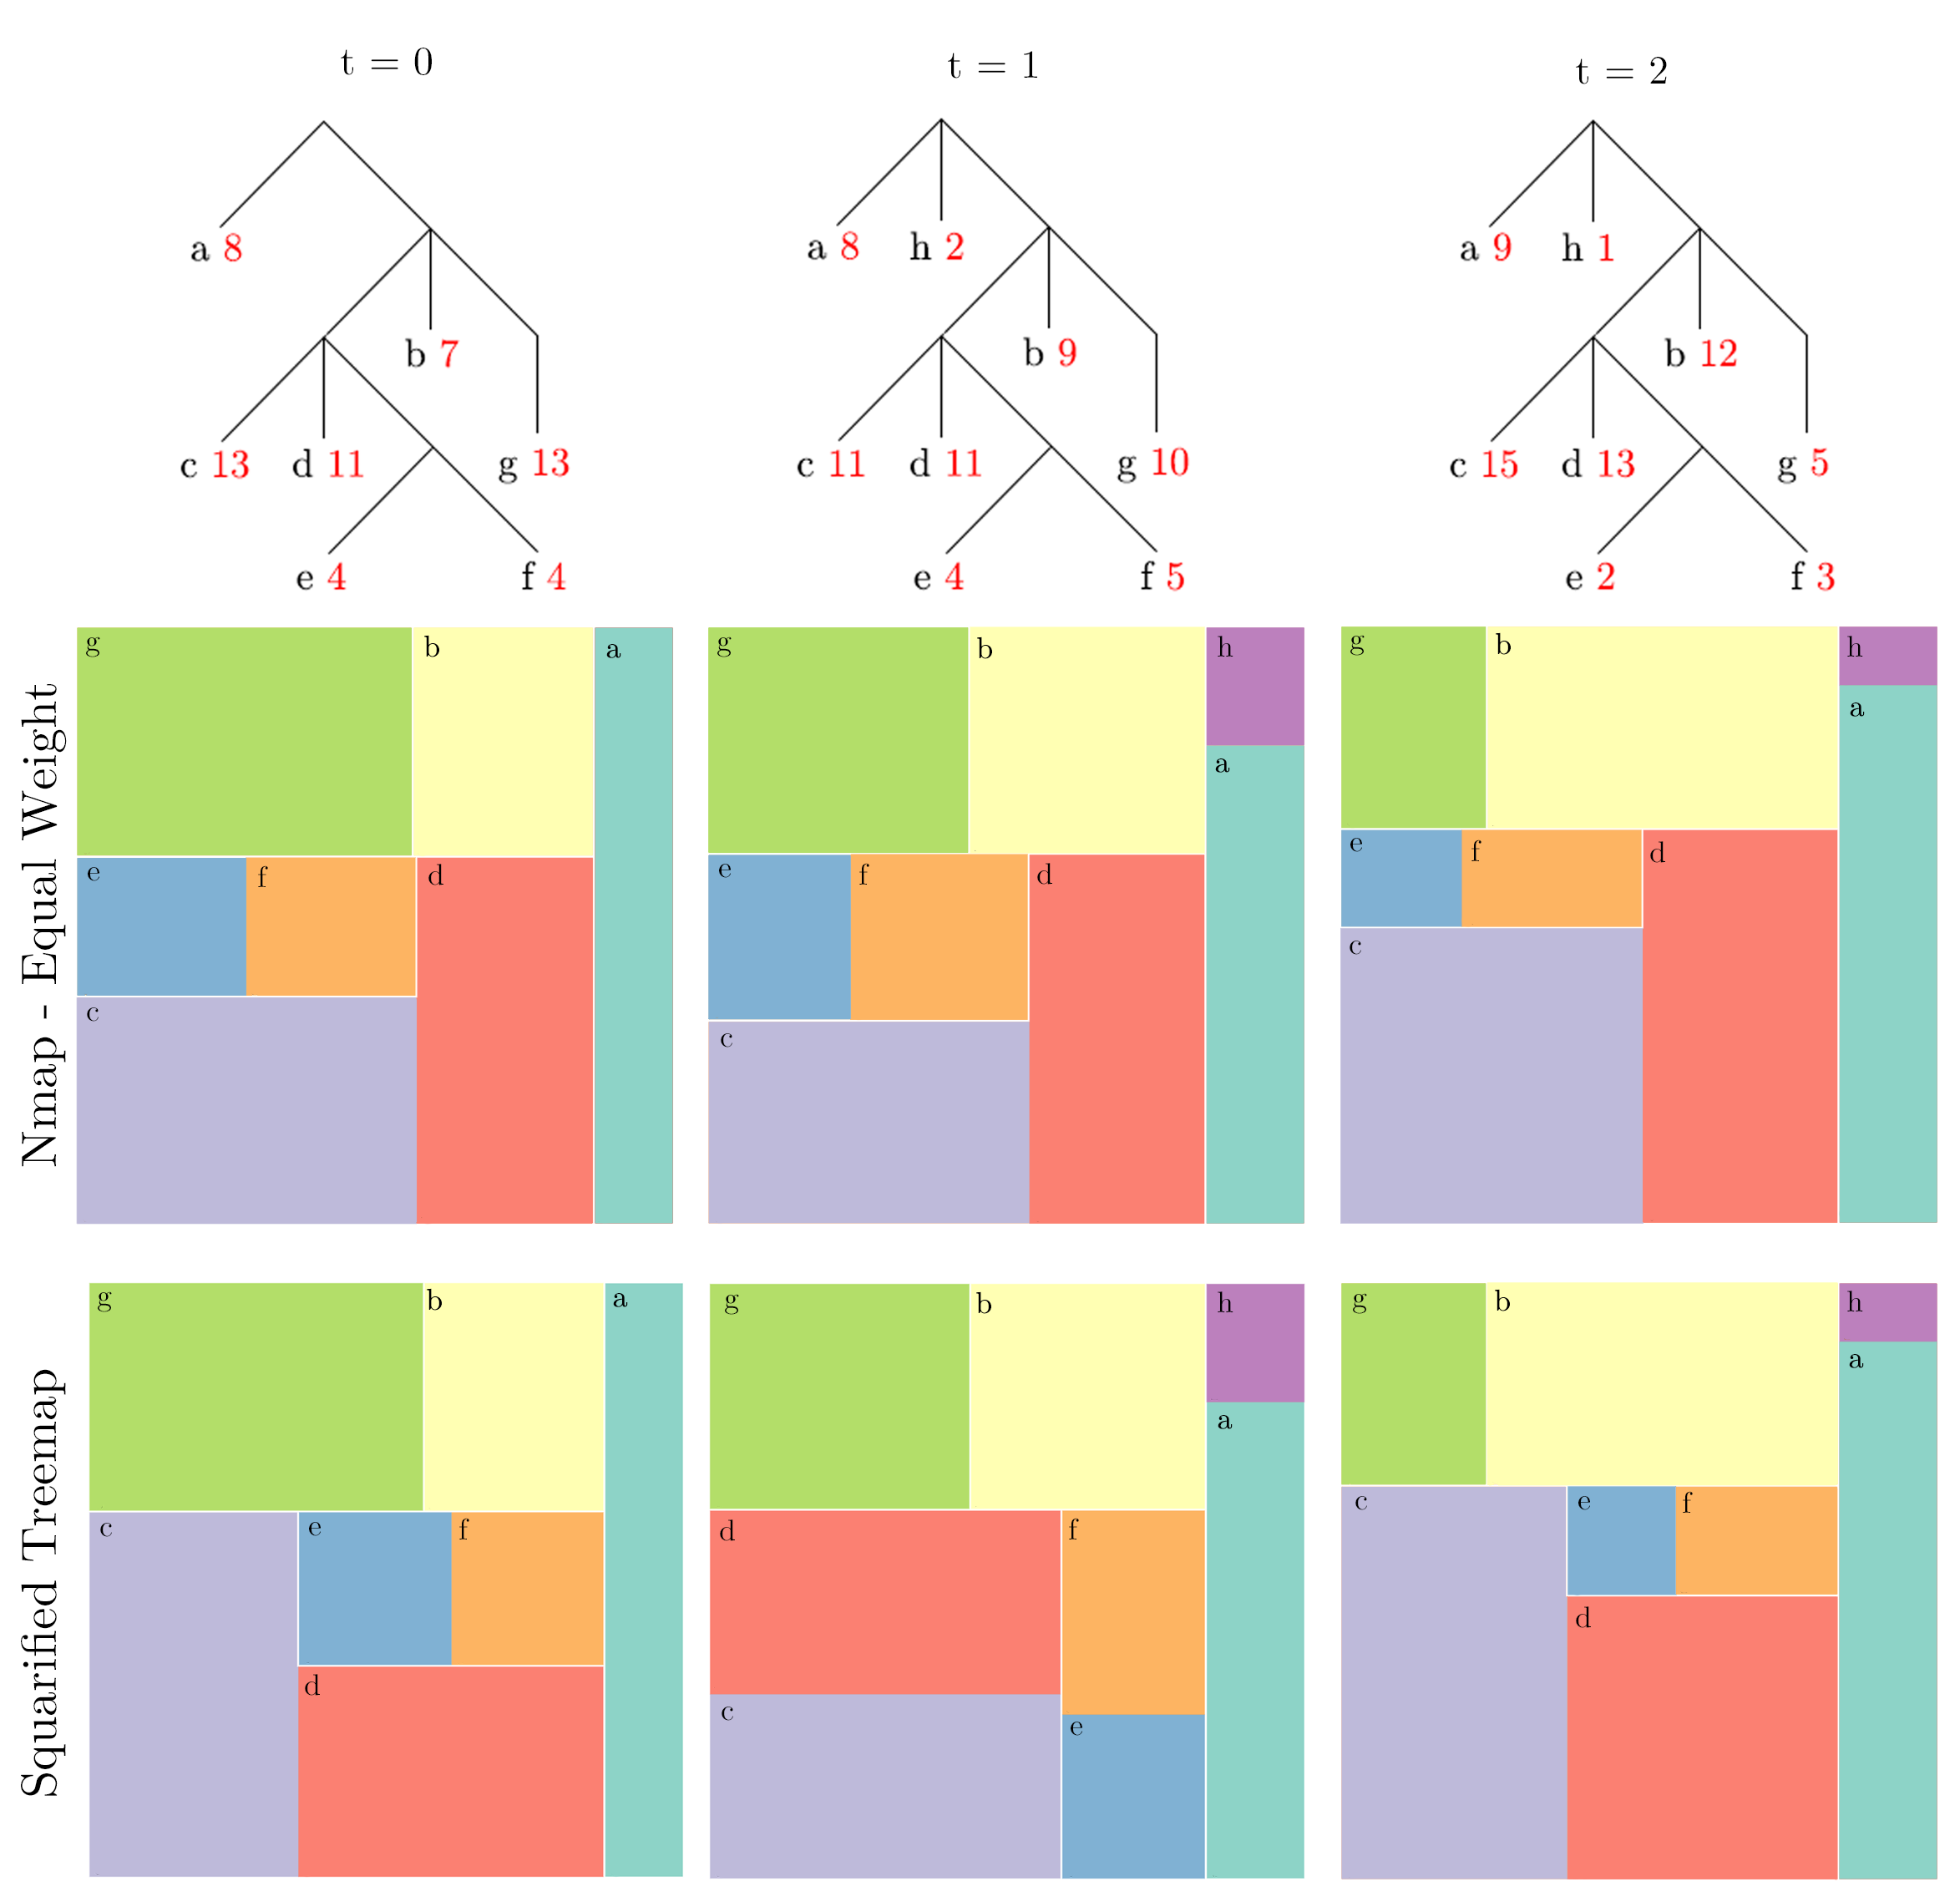
\includegraphics[width=\linewidth]{figures/intro/mov_sub_new.png}
    \caption{Layouts generated by NMap Equal Weight and Squarified Treemaps for a sample dataset
    of 3 time steps. We see how the former is more stable, and similar in aspect ratio, than/as the
    latter.}
    \label{fig:intro-tm-demo-instability}
\end{figure*}

To create faithful and useful representation of temporal data, we need to be able to ensure temporal coherence. Small changes in the data should result in small changes in the visualization, and no large changes in the visualization should be induced by the algorithmic artifacts, that is, we want to guarantee that changes perceived by the viewer are due to changes in the data alone.


\section{Objectives and contributions}

We have established that treemaps and projections are essential tools for making sense of hierarchical and multidimensional data, respectively. However, when it comes to applying these visual encodings to time-dependent data, these methods tend to show undesirable traits and not a lot of research effort has been dedicated to understanding, testing, and developing methods that preserve temporal coherence. This research gap leads us to this thesis' high-level research question.

\subsection*{How to extend projections and treemaps to stably, accurately, and scalably handle temporal multivariate and hierarchical data?}

To address this question, there are three components that must be satisfied in either track. We must be able to:

\subsection*{A. Develop ways of accurately measuring instability}

To evaluate the stability of a dynamic treemap or dynamic projection, we need to have reliable measurement tools that quantify the relationship between data change and visual change.

For treemaps, we developed the \emph{Unavoidable Change} metric, based on the mathematically proven minimum change that cells would need to undergo to accommodate the data change, and \emph{Baseline Treemaps}, a similar method to approximate the minimum amount of change that any time-dependent treemap must incur when data changes. We also proposed a set of stability metrics for dynamic projections based on the mathematics of visual quality metrics.

Before these, there were no methods designed to measure instability that took into consideration data change -- they only looked at visual change, which can be deceiving.


\subsection*{B. Evaluate methods in the literature considering the tradeoff between stability and visual quality}

We produced comprehensive evaluations for dynamic treemaps and projections.
This entailed work in the following axes:

\begin{itemize}
    \item \emph{Metrics:} We proposed and implemented a novel set of metrics that reliably measures visual quality and stability.
    \item \emph{Datasets:} Since there was no previous extensive evaluation or benchmark designed for testing dynamic treemaps or projections, it was necessary to collect/generate the set of datasets that drove the evaluations. 
    \item \emph{Methods:} Collection, implementation, and proposal of several dynamic treemap and projection algorithms. Most of the work on the topic up until then was conjectural and not quantitatively tested.  
    \item \emph{Analysis:} Combine the previous axes into comprehensive insight into dynamic projections and treemaps.
\end{itemize}

\subsection*{C. Design state-of-the-art methods that strike good balance between stability and visual quality}

Once the tools necessary to test and compare dynamic treemaps and projections were in place, we were able to leverage the gained insights to produce state-of-the-art algorithms that strike great balance between stability and visual quality.

We have developed Greedy Insertion Treemap (GIT), a stable and scalable state-aware method.

Regarding projections, we proposed PCD-tSNE and LD-tSNE, which are neighborhood-based methods that use global guides to steer projection points. This avoids unstable movement that does not encode data dynamics while keeping t-SNE's neighborhood preservation ability.

The other most effective techniques for dynamic projections are Autoencoder-based and Global PCA. Though we cannot claim that these are part of our contribution, we believe we were the first to shed light on their effectiveness in the context of temporal data.  

\bigbreak

Lastly, it is important to mention that all aspects of our research are open. All the code and data is organized and available online to facilitate further research on dynamic treemaps and projections. 

\section{Organization of the thesis}


\eduardo{will add refs later}

\eduardo{(explanation for unavoidable change metric is not in the text yet -- software visualization paper)}

\eduardo{quotes come from here http://www.cs.umd.edu/hcil/treemap-history/index.shtml}